\clearpage
\section{Definitionen}

In diesem Kapitel werden Begrifflichkeiten erklärt, die für die Recherchen der Online-Bezahldienste und deren marktwirtschaftlichen Analyse von Nutzen sein können. 

\subsection[E-Payment]{E-Payment\footnote{\url{ https://de.wikipedia.org/wiki/Elektronisches_Geld}}}

E-Payment steht für Electronic Payment und bezeichnet eine neue Erscheinungsform des Geldes. Die offizielle Definition in Europa lautet:
\begin{quote}
``E-Geld-Richtlinie, 2000/46 EG: ein monetärer Wert in Form einer Forderung gegen die ausgebende Stelle, der
\begin{itemize}
	\item auf einem Datenträger gespeichert ist,
	\item gegen Entgegennahme eines Geldbetrags ausgegeben wird, dessen Wert nicht geringer ist als der ausgegebene monetäre Wert,
	\item von anderen Unternehmen als der ausgebenden Stell als Zahlungsmittel akzeptiert wird.''
\end{itemize}
\end{quote}



\subsubsection{Erscheinungsformen von E-Geld}

\paragraph{Karten gestütztes E-Geld}oder auch Kartengeld genannt, beinhaltet das E-Geld auf einer Karte mit Chip oder Magnetstreifen. In Deutschland ist die Geldkarte\footnote{\url{  https://de.wikipedia.org/wiki/Geldkarte}} das bekannteste Beispiel. Auf der Chipkarte ist das Guthaben gespeichert, welches dann zur Bezahlung verwendet werden kann.

\paragraph{Software basiertes E-Geld}bzw. Netzgeld wird über ein Rechnernetz transferiert. Das E-Geld befindet sich entweder auf einer Festplatte oder einem Online-Konto, welches dann zwischen zwei Rechnern transferiert wird. Der Online-Bezahl-Dienstleister PayPal transferiert Netzgeld mittels Online-Konten der jeweiligen registrierten Benutzer.
%https://de.wikipedia.org/wiki/Elektronisches_Geld

\subsubsection{Elektronische Zahlungssysteme}
%https://de.wikipedia.org/wiki/Elektronisches_Geld
Kategorisieren lassen sich elektronische Zahlungssysteme nach folgenden Betrachtungsweisen:
\paragraph{Zeitpunkt}
\begin{itemize}
     \item Prepaid: Zahlung wird vor dem Kauf ausgeführt
     \item Pay Now: Zahlung bzw. Abbuchung vom Kundenkonto wird zeitgleich mit dem Kauf ausgeführt
     \item Pay Later: Kundenkonto wird erst nach der Transaktion belastet.
\end{itemize}

\paragraph{Höhe des Betrags}
\begin{itemize}
     \item Macropayment: Zahlungen ab ca. \EUR{5}
     \item Micropayment: Zahlungen von ca. \EUR{0.05} bis ca. \EUR{5}
     \item Milipayment bzw. Minipayment: Zahlungen bis ca. \EUR{0.05}
\end{itemize}

\paragraph{Eingesetzter Hard- und Software:} Kategorisieren nach den eingesetzten Hard-/Software-Komponenten

\paragraph{Mischkategorisierung}
Die Kategorisierung reicht heutzutage nicht mehr aus, um die E-Payment-Systeme überschaubar abzugrenzen. Sie vermischen sich in den Kategorien zu sehr. Um die Dienstleister weitestgehend über\-sichtlich abzugrenzen, entwickelte Knud Bähle die folgende Mischkategorisierung:
\\
%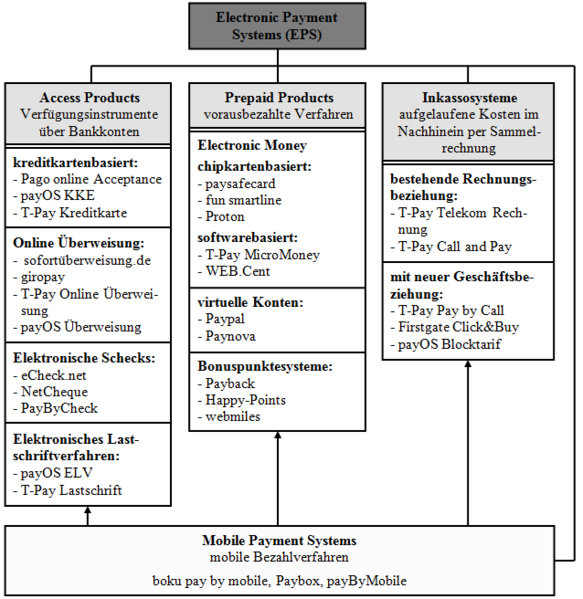
\includegraphics[]{img/Mischform.png}

\paragraph{Access Products} führen ihre Zahlungen über reale Bankkonten. Der Kunde gibt die benötigten Informationen seines Bankkontos an den Dienstleister. Online-Zahlungen mittels Kreditkarten, elektronischer Schecks oder Lastschriftverfahren führen auf das beschriebene Bankkonto zurück.

\paragraph{Prepaid Products} bieten E-Geld an, welches gegen reales Geld getauscht wird. Der Kunde hat somit sein reales Guthaben für Online-Zahlungen als E-Geld zur Verfügung stehen. Das Guthaben bzw. das E-Geld ist dann in Form von Chipkarten, Netzgeld oder auf einem virtuellem Konto gespeichert.

\paragraph{Inkassosysteme} schicken aufgelaufene Kosten nach Transaktionen per Sa\-mmelrechnung. 

\paragraph{Mobile Payment Systems} sind Bezahlsysteme, bei welchem Beträge über Mobilfunktelefone beglichen werden können. Klingeltöne oder Bilder, die man über eine SMS an den jeweiligen Anbieter als Bestellung gesendet hat, wird von der PrePaid-Karte abgebucht oder bei Mobilnetzverträgen auf die Rechnung hinzu addiert.\footnote{\url{ https://de.wikipedia.org/wiki/Handypayment}}



\subsection[Die Vision eines Unternehmens]{Die Vision eine Unternehmens\footnote{\url{ http://www.sunternehmensentwicklung.de/vision-unternehmen/uncategorised/vision-unternehmen.html}}}

Eine Unternehmensvision beschreibt ein in der Zukunft liegenden erstrebenswerten Zustand bzw. die zukünftige Entwicklung des Unternehmens. Sie erzielt je nach Betrachtungsweise verschiedene Effekte: Die Mitarbeiter des Unternehmens identifizieren sich mit der Vision und dem Unternehmen selbst. Die Langfristigen Ziele des Unternehmens sollen für jeden Mitarbeiter allgegenwärtig sein und den Sinn der eigenen Tätigkeit bewusst machen. Es fördert somit die Motivation und den Spaß an der Arbeit. Bei Kunden weckt eine Vision das Interesse an ein Unternehmen und verleiht einen souveränen Eindruck: Die Vision vermittelt Vertrauen.
 

\subsection[Geschäftsmodell]{Geschäftsmodell\footnote{\url{ http://de.wikipedia.org/wiki/Geschaeftsmodell}}}

Ein Geschäftsmodell ist eine modellhafte Beschreibung über die logische Funktionsweise eines Unternehmens. Es beantwortet folgende Fragen hinsichtlich der drei Hauptkomponenten:
\begin{itemize}
	\item Nutzerversprechen: Welchen Nutzen und Wert stiftet das Unternehmen für Kunden und seinen strategischen Partnern?
	\item Architektur der Wertschöpfung: Wie erbringt das Unternehmen diesen Nutzen?
	\item Ertragsmodell: Wodurch erwirtschaftet das Unternehmen seine Gewinne?
\end{itemize}

Geschäftsmodelle helfen bei der Analyse des Unternehmens. Es kann Schlüsselfaktoren herausfinden und die Gründe für einen Erfolg oder Misserfolg eines Unternehmens erklären.


\subsection[Kernkompetenz]{Kernkompetenz \footnote{\url{ http://de.wikipedia.org/wiki/Kernkompetenz}}}

Unter einer Kernkompetenz versteht man eine Fähigkeit eines Unternehmens, die im Vergleich zur Konkurrenz besser ausgeführt wird und dadurch einen Wettbewerbsvorteil erlangt. Jedes Unternehmen besitzt eine Kernkompetenz, auf welches es sich stützt und versucht, diese weiter auszubauen. Je nach Unternehmenslage kann ein Unternehmen seine Kernkompetenzen aus- oder abbauen oder auch das Repertoire an Kernkompetenzen erweitern oder verringern.
\subsubsection{Kernkompetenzen identifizieren}
Kernkompetenzen können identifiziert werden. Um diese zu finden, können folgende Eigenschaften einer angeblichen Kernkompetenz untersucht werden:
\begin{itemize}
\item Differenzierung: besitzt die Kernkompetenz das Potential, einen nachhaltigen Vorteil gegenüber der Konkurrenz zu führen?
\item Diversifikation: bietet die Kernkompetenz Zugang zu neuen Märkten?
\item Kundennutzen: hat der Kunde einen nachhaltigen Mehrwert durch diese Kernkompetenz?
\item Imitationsschutz: kann die Kernkompetenz von der Konkurrenz leicht imitiert werden?
\end{itemize}




\subsection[Kritischer Erfolgsfaktor]{Kritischer Erfolgsfaktor \footnote{\url{ http://de.wikipedia.org/wiki/Kritischer_Erfolgsfaktor}}}

Kritische Erfolgsfaktoren sind Eigenschaften, die bei einem Unternehmen bei guten Werten das Erreichen ihrer Ziele ermöglicht. Sie entscheiden über den Erfolg eines Unternehmens. In einem IT-Projekt entscheiden gutes Projekt- und Risikomanagement, sowie auch das Entwicklungsteam zum Erfolg des Projektes selbst und somit auch der des Unternehmens.



\subsection[Strategie]{Strategie\footnote{\url{ http://de.wikipedia.org/wiki/Strategie_(Wirtschaft)}}}
Eine Strategie im Wirtschafts-Kontext ist eine geplante Verhaltensweise eines Unternehmens um ihre Ziele zu erreichen. Sie legt fest, in welchen Aktivitätsfelder das Unternehmen tätig sein soll. Strategien richten sich auf das gesamte Unternehmen und spiegeln die zentrale Einstellungen, Wünsche und Wertvorstellungen der bestimmenden Entscheidungsträger des Unternehmens wider. Es bezieht sich auf das Umfeld und der Konkurrenz: Soll eine Fusion mit der Konkurrenz erfolgen? Gibt es eine Möglichkeit, sich von der Konkurrenz abzugrenzen? Kann man Kernkompetenzen der Konkurrenz imitieren? 



\subsection[Indikatoren]{Indikatoren\footnote{\url{ http://de.wikipedia.org/wiki/Indikator_(Wirtschaft)}}}

Indikatoren sind im Allgemeinem Messgrößen, die zur Steuerung und Orientierung einer Organisation helfen. Sie beschreiben einen Zustand oder quantifizierbaren Wert. In der Wirtschaft unterscheidet man zwischen volkswirtschaftlichen und betriebswirtschaftlichen Indikatoren bzw. Kennzahlen.

\subsubsection{Volkswirtschaftlicher Indikator [9]}

Volkswirtschaftliche Indikatoren werden auch Konjunkturindikatoren oder makroökonomische Kennzahlen genannt. Ihre Werte beschreiben die wirtschaftliche Situation im Allgemeinen von Volkswirtschaften und können als Basis für die Erstellung von Wirtschafts-Prognosen eingesetzt werden. 
\\
Konjunkturindikatoren eignen sich zur Bewertung von Aktien, weil sie Rück\-schlüsse aus der gesamtwirtschaftlicher Entwicklung ziehen, die wiederum die wirtschaftliche Situation einzelner Industriesektoren abbilden. Konjunkturindikatoren lassen sich in drei Kategorien aufteilen:

\paragraph{Mengenindikatoren} informieren über die Mengenentwicklung eines Bezugsobjektes, wie zum Beispiel Arbeitslosenzahl, Auftragseingänge oder Industrieproduktion.
\paragraph{Preis- bzw. Kostenindikatoren} beschreiben das Preisniveau bzw. die Entwicklung eines Bezugsobjektes. Dazu gehören Aktienkurse, Immobilienpreise, Lebensmittelpreise und Rohstoffpreise.
\paragraph{Früh-, Präsenz- und Spätindikatoren} beschreiben den zeitlichen Vor- bzw. Nachlauf eines Sachverhaltes. 

Frühindikatoren weisen auf zukünftige Entwicklung der Wirtschaftslage. Dazu gehören der Aktienindex, Rohstoffindex, Gewinnerwartungen und Einzelhandelsumsätze. 

Präsenzindikatoren geben Auskunft über die aktuelle Wirtschaftsentwicklung: Bruttoinlandsprodukt, Industrieproduktion, Kurzarbeit und Lagerbe\-stände.

Spätindikatoren beschreiben die Wirtschaftsentwicklung in der Vergangenheit: Arbeitslosenquote, Inflationsrate, Insolvenzen, Lohnentwicklung, Steu\-ereinnahmen des Staates.

\paragraph{Wachstumsrate} bzw. Inflationsrate stellen absolute Größen dar, wie den Stand eines Aktienindex, Logistikindex oder Rohstoffindex.
   

\subsubsection[Betriebswirtschaftlicher Indikator]{Betriebswirtschaftlicher Indikator \footnote{\url{http://de.wikipedia.org/wiki/Betriebswirtschaftliche_Kennzahl}}}
Betriebswirtschaftliche Indikatoren dienen zur Beurteilung von Unternehmen innerhalb der Betriebswirtschaft. Folgende Funktionen können diese Kennzahlen besitzen:

\paragraph{Entscheidungsfunktion:} Entscheidungsträger können anhand von Kennzahlen betriebswirtschaftliche Entscheidungen treffen. Kennzahlen können auf Probleme oder Chancen hinweisen.
\paragraph{Kontrollfunktion:} Kennzahlen können der Kontrolle des Gesamterfolges des Unternehmens dienen.
\paragraph{Koordinationsfunktion:} helfen bei der Durchsetzung von Entscheidungen über die Koordination verschiedener unternehmerischer Bereiche und bei der Verhaltenssteuerung von Mitarbeitern.
\paragraph{Verhaltenssteuerungsfunktion:} zum Motivieren der Mitarbeiter zu einer für das Unternehmen positiven Verhaltensweise.

\newpage

\paragraph{Arten von Kennzahlen}
\subparagraph{Absolute Kennzahlen} drücken einen betriebswirtschaftlichen Einzelwert aus. Sie stehen in keine Relation zu anderen Kennzahlen. Zu diesen Arten von Kennzahlen gehören beispielsweise Summenwerte, Differenzwerte und Mittelwerte.
\subparagraph{Relative Kennzahlen} entstehen durch eine Relation zweier betriebswirtschaftlicher Werte zu einer Kennzahl, die einen erhöhte oder spezifische Aussagekraft besitzt.

\subsubsection{Gliederung von betriebswirtschaftlichen Kennzahlen}
Kennzahlen lassen sich nach dem zugrunde liegenden Sachverhalt, der durch sie ausgedrückt werden soll, gliedern.

\paragraph{Erfolgskennzahlen} dienen der Ermittlung des Unternehmenserfolgs und orientieren sich am Gewinn oder am Unternehmenswert. Zu Erfolgskennzahlen gehören Umsatz, Cashflow, Produktergebnis,, Gesamtbetriebsertrag, Rohertrag und Gewinne vor Steuern.

\paragraph{Liquiditätskennzahlen} geben Informationen über den Zustand der Zahlungsmöglichkeit eines Unternehmens an, um seine fälligen Verbindlichkeiten begleichen zu können. Kennzahlen wie Cash Ratio, Anlagendeckung und Einzugsliquidität gehören zu Liquiditätszahlen.\footnote{\url{http://www.wirtschaftslexikon24.com/d/liquiditaetskennzahlen/liquiditaetskennzahlen.htm}}


\paragraph{Rentabilitätskennzahlen} beschreiben das Verhältnis einer Erfolgsgröße zum eingesetztem Kapital: Gesamtkapitalrentabilität, Eigenkapitalrentabilität und Umsatzrendite. \footnote{\url{http://de.wikipedia.org/wiki/Rentabilitaet}}

\paragraph{Bilanzkennzahlen} oder Kennzahlen zur Kapitalstruktur geben Auskunft über die Bilanz eines Unternehmens, zum Beispiel Eigenkapitalquote, Fremdkapitalquote, Verschuldungsgrad und Anlagenintensität.

\paragraph{Kennzahlen zur Umschlagshäufigkeit} wie Kapital- und Lagerumschlags\-häuigkeit, beschreiben, wie oft ein Wert sich in einem bestimmten Zeitraum wiederholt.
    
 



\subsection[Marktanalyse]{Marktanalyse \footnote{\url{http://de.wikipedia.org/wiki/Marktanalyse}}}

Die Marktanalyse dient der Darstellung der aktuellen Marktsituation. Es werden Daten erhoben, die gerade aktuell sind und so für Entscheidungen herangezogen werden können. Die Daten stammen aus internen Marktdaten, wie Verkaufszahlen oder Produktionskosten und externen Marktdaten wie makroökonomische Trends. Aus der Analyse können Marketingpläne erstellt werden, aus denen strategische Ziele und Maßnahme abgeleitet werden können.
\\
Zu Marktanalysen gehören folgende Recherchen dazu:
\begin{itemize}
	\item Marktpotential bei innovativen Produkten oder Dienstleistungen
	\item Marktvolumen und Marktentwicklung
	\item Marktstruktur nach Teilmärkten in Regionen/Ländern, Produktgruppen oder Kundentypen
	\item Konkurrenzanalyse
	\item Produktlebenszyklusanalyse 
\end{itemize}



\subsection[Konkurrenzanalyse]{Konkurrenzanalyse \footnote{\url{http://de.wikipedia.org/wiki/Konkurrenzanalyse}}}
In der Konkurrenzanalyse werden Informationen über Konkurrenzunternehmen systematisch und legal gesammelt und ausgewertet. Dabei werden ihre Produkte, Marktentwicklungen, neue Patente und Technologien beobachtet und analysiert. Es ist ein wichtiger Bestandteil der Marktanalyse und ermöglicht Unternehmen eine frühzeitige Anpassung ihrer Strategie um somit Wettbewerbsvorteile zu erreichen.
